\section{Quickly computing certain entries of a thin matrix product}\label{sec:result}

We now present our main new algorithm, for computing a subset of the output entries of a thin matrix product. We call such a matrix product \emph{thin} since the input matrices are highly rectangular. We work in the standard word RAM model with $O(\log N)$-bit words, and thus count operations on $O(\log N)$-bit integers.

\begin{theorem}\label{thm:main}
Let $D\ge4$ be a power of four and $N\ge D^{18}$. Given as input matrices $X\in\Z^{N\times D}$ and $Y\in\Z^{D\times N}$, whose entries are integers of absolute value at most $N^{O(1)}$, as well as a set $W$ of at most $N^2/\sqrt D$ positions of an $N \times N$ matrix, the entries $(XY)[I,J]$, $(I,J)\in W$, can be computed deterministically in time $O(N^2\log^2\!D/D^{1/18})$.
\end{theorem}

We call the positions in $W$, and the entries of $XY$ at them, \emph{wanted}. We emphasize that $X, Y$, and $XY$ may be arbitrary dense matrices, and no structure is assumed about the set $W$ other than its size $|W| \leq N^2/\sqrt D$. 

We have aimed to present this section in a way that is accessible to nonexperts. Some details in Theorem~\ref{thm:main}, such as the exponent $18$, are chosen to simplify the presentation in this section while still proving a version sufficient to refute the $3$SUM and APSP hypotheses. Later, in Section~\ref{sec:general}, we present a stronger data structure version that has improved parameter trade-offs.

Notably, while the language of tensors and bilinear complexity naturally describes much of our algorithm and the prior work it builds on, we deliberately avoid that language here. This is in part so that a reader unfamiliar with that background may still follow, but also because our arguments here will focus on sparsity and combinatorial properties of our algorithms and algebraic identities that are often intentionally abstracted away in tensor language.

Sections~\ref{sec:background}--\ref{sec:full} present an exposition of the relevant prior work that we directly build on, especially Strassen~\cite{Str69},  Sch\"onhage~\cite{Sch81}, and Coppersmith~\cite{Cop82}, and no prior understanding of those works is assumed. The main new idea of this paper is then presented in Section~\ref{sec:sparse}. 

\paragraph{Technique overview.}
Strassen's algorithm multiplies matrices by applying a small identity (seven products for multiplying $2\times2$ matrices) recursively. In that algorithm, the multiplications happen at the leaves of a recursion tree, and the additions that prepare the leaves (the ``encoding phase'') and assemble the result (the ``decoding phase'') are comparatively cheap. We do the same with an identity of Sch\"onhage that computes, simultaneously, two small rectangular matrix products. Applied at $L$ levels of recursion, the identity computes $2^L$ matrix products at once. In order to multiply $X$ and $Y$ using this, we cut them into smaller blocks, and then simultaneously multiply many pairs of blocks using Sch\"onhage's identity (Section~\ref{sec:full}).

The new idea (Section~\ref{sec:sparse}) is to visit only the leaves of the recursion tree that the wanted entries from $W$ need. A priori, it is not clear that this reduces the number of leaves by much, or that the encoding and decoding phases stay cheap. Both nonetheless turn out to hold, for two reasons.

First, we observe that the additions in the encoding phase that prepare the leaves depend on $X$ alone or on $Y$ alone (as is the case in all tensor rank decompositions). Since each $X$ block is multiplied with every $Y$ block, we only need to compute these additions once for each $X$ block and may share them among many calls to our algorithm (and similarly for $Y$). One reason for the requirement $N\ge D^{18}$ is to ensure that this total cost will be negligible (Section~\ref{sec:encoders}).

Second, we prune the recursion tree, and make a recursive call only when one of its outputs is wanted by $W$. This way, the running time is governed by the union of the sets of leaves that the wanted entries need. Most of the analysis goes into bounding this union (Section~\ref{sec:counts}). We will see that every output entry has a private leaf that no other entry needs, but that all its other leaves are shared by many entries. We will characterize each leaf by how often one needs to pick each of the two matrix products from Sch\"onhage's identity to get to it in the recursion tree, and find a trade-off: choosing one of the matrix products leads to a relatively small number of leaves, while choosing the other increases how many output entries share each leaf. Balancing the two, we will find that a set of $N^2/\sqrt D$ wanted entries only needs about $N^2/D^{1/18}$ leaves in all, and paying $O(\log^2\!D)$ operations per leaf gives Theorem~\ref{thm:main}.

\subsection{Strassen's recursive algorithm}\label{sec:background}

We use the recursive approach for multiplying matrices introduced by Strassen~\cite{Str69}. We begin by recalling his algorithm for intuition. The key behind his algorithm is an identity that shows how to multiply two $2\times2$ matrices $A$ and $B$ using only seven multiplications instead of eight. It forms seven products, each of a linear combination of the entries of $A$ with a linear combination of the entries of $B$, and then obtains each entry of $AB$ as a linear combination of those seven products. Recall that, writing $A=(a_{ij})$ and $B=(b_{ij})$, the seven products are
\begin{equation}\label{eq:strassen}
\begin{alignedat}{2}
S_1&=(a_{11}+a_{22})(b_{11}+b_{22}), &\qquad S_5&=(a_{11}+a_{12})\,b_{22},\\
S_2&=(a_{21}+a_{22})\,b_{11}, & S_6&=(a_{21}-a_{11})(b_{11}+b_{12}),\\
S_3&=a_{11}\,(b_{12}-b_{22}), & S_7&=(a_{12}-a_{22})(b_{21}+b_{22}),\\
S_4&=a_{22}\,(b_{21}-b_{11}),
\end{alignedat}
\end{equation}
and the product is
\[
AB=\begin{pmatrix} S_1+S_4-S_5+S_7 & S_3+S_5\\ S_2+S_4 & S_1-S_2+S_3+S_6\end{pmatrix}.
\]
To use this identity to multiply $N \times N$ matrices $A, B$ for larger $N$, we interpret $A$ and $B$ as $2\times2$ block matrices (whose entries are $N/2 \times N/2$ matrices), then multiply them as in the identity, i.e., we form seven pairs of linear combinations of the blocks of $A$ and of $B$, recursively multiply each pair, and then assemble the four blocks of $AB$ from the seven results. When $N=2^L$, the recursion tree (Figure~\ref{fig:strassen}) has $L$ levels, and $7^L$ leaves, one for each choice of one of the seven products at each level. The multiplications take place at the leaves, meaning there are $7^L=N^{\log_27} < N^{2.81}$ multiplications in total. We call the additions on the way down, which prepare the leaves and are computed from $A$ alone and from $B$ alone, the \defn{encoding}, and those on the way up, which assemble the product, the \defn{decoding}.

\begin{figure}[tb]
\centering
\begin{tikzpicture}[x=1cm,y=1cm,
  call/.style={draw,rounded corners=1pt,inner sep=2pt,font=\scriptsize,minimum height=4mm,fill=blue!8},
  small/.style={draw,rounded corners=0.5pt,inner sep=0pt,minimum height=2.6mm,minimum width=1.3mm,fill=blue!8},
  leafn/.style={draw,inner sep=0pt,minimum height=2mm,minimum width=1.1mm,fill=orange!30},
  wire/.style={gray!70,line width=0.35pt},
  lab/.style={font=\scriptsize,align=center}]
\node[call] (root) at (6,4.3) {$N\times N$};
\foreach \i in {0,...,6} {
  \node[call] (c\i) at (0.9+1.7*\i,2.9) {$\tfrac N2\times\tfrac N2$};
  \draw[wire] (root.south) -- (c\i.north);
  \foreach \j in {0,...,6} {
    \node[small] (d\i\j) at (0.9+1.7*\i+0.19*\j-0.57,1.95) {};
    \draw[wire] (c\i.south) -- (d\i\j.north);
  }
  \node[font=\scriptsize] at (0.9+1.7*\i,1.45) {$\vdots$};
}
\foreach \k in {0,...,58} { \node[leafn] at (0.33+0.1955*\k,0.95) {}; }
\node[lab] at (6,0.5) {$7^L$ leaves: products of two numbers};
\node[lab] at (1.9,4.3) {$\downarrow$ on the way down: seven pairs of\\ linear combinations of the blocks (encoding)};
\node[lab] at (10.1,4.3) {$\uparrow$ on the way up: the four blocks of\\ the product from the seven results (decoding)};
\end{tikzpicture}
\caption{Strassen's recursion on $N\times N$ matrices, $N=2^L$, showing the first two levels of calls below the root.}
\label{fig:strassen}
\end{figure}

To calculate the total cost of Strassen's algorithm, we also need to count the additions and subtractions at the internal vertices of the recursion tree. At depth $k$ of the recursion tree, there are $7^k$ internal vertices. Both on the way down and on the way up the tree, the algorithm must compute linear combinations of $2^{L-k}\times2^{L-k}$ matrices at each of these vertices, which uses $O(4^{L-k})$ operations. The total across the whole tree is therefore $\sum_{k=0}^{L-1}7^k4^{L-k}=O(7^L)$, a geometric series dominated by its last term, so the additions only increase the running time by a constant factor. This phenomenon is prevalent in recursive matrix multiplication algorithms, although in the new algorithm we develop in Section~\ref{sec:sparse} below, this same argument will no longer apply, and we will need to count the additions and subtractions more carefully.

\subsection{Sch\"onhage's identity for an inner product and an outer product}\label{sec:identity}

While we will still use Strassen's recursive approach here, we will replace his identity with another one due to Sch\"onhage~\cite{Sch81}. In this subsection we give the notation to introduce this identity and explain its usefulness.

It will be convenient to write such identities as trilinear polynomials.\footnote{These are often called tensors, or order-3 tensors, in the literature.} As an example, we first show how to write Strassen's identity from Section~\ref{sec:background} in this way. Introduce four \defn{output variables} $c_{11},c_{12},c_{21},c_{22}$, one for each entry of the product $AB$, and multiply each of the seven products $S_1,\dots,S_7$ of Strassen's identity above by the signed sum of the output variables of the entries where it appeared in the decoding phase. For instance, $S_1$ appears in the formulas for $(AB)_{11}$ and $(AB)_{22}$, so it is multiplied by $c_{11}+c_{22}$, and $S_5$ appears in the formula for $(AB)_{11}$ with a minus sign and in the formula for $(AB)_{12}$, so it is multiplied by $c_{12}-c_{11}$. Strassen's identity then reads
\begin{multline*}
S_1(c_{11}+c_{22})+S_2(c_{21}-c_{22})+S_3(c_{12}+c_{22})+S_4(c_{11}+c_{21})\\
+S_5(c_{12}-c_{11})+S_6\,c_{22}+S_7\,c_{11}\;=\;\sum_{i,j,k=1}^{2}a_{ij}\,b_{jk}\,c_{ik},
\end{multline*}
where $S_1,\dots,S_7$ are the products of two linear forms from~\eqref{eq:strassen}. Now the coefficient of $c_{ik}$ on the right-hand side is the entry $(AB)_{ik}=a_{i1}b_{1k}+a_{i2}b_{2k}$ that we want, and its coefficient on the left-hand side is the combination of the seven products that computes it, such as $S_1+S_4-S_5+S_7$ for $c_{11}$. This polynomial identity thus records the linear combinations and products to be formed, as well as the combinations that assemble the outputs from them.

We will next present Sch\"onhage's identity in the same way. 
Recall that the \defn{outer product} of two vectors $(x_1,x_2,x_3)$ and $(y_1,y_2,y_3)$ consists of the nine numbers $x_iy_j$, and the \defn{inner product} of two vectors $(p_{11},p_{12},p_{21},p_{22})$ and $(q_{11},q_{12},q_{21},q_{22})$ is the single number $\sum_{i,j=1}^{2}p_{ij}q_{ij}$. These are special cases of matrix products: the outer product is multiplying a $3\times1$ matrix times a $1\times3$ matrix, and the inner product is multiplying a $1\times4$ matrix times a $4\times1$ matrix. (We index the $p$ and $q$ variables with $\{1,2\} \times \{1,2\}$ rather than $\{1,2,3,4\}$ to set up nicer notation for $\hat{p}$ and $\hat{q}$ in Lemma~\ref{lem:identity} below.)

Separately computing the inner product and outer product would use $9 + 4 = 13$ multiplications. However, Sch\"onhage~\cite[\S6, eq.~(6.3), with $k=n=3$]{Sch81} showed that they can be computed (along with some error terms that will turn out to be harmless) using only 10 multiplications. The fact that this is possible even when the inner and outer products are on disjoint sets of variables is surprising, and refuted a border rank version of the ``direct sum conjecture for tensor rank''~\cite{Str73}.

We call $x_1,x_2,x_3,\allowbreak p_{11},p_{12},p_{21},p_{22}$ the seven \defn{left variables} and $y_1,y_2,y_3,\allowbreak q_{11},q_{12},q_{21},q_{22}$ the seven \defn{right variables}. We will also use ten output variables $z_{ij}$ (for $1 \leq i,j \leq 3$) and $z_0$, one for each of the ten quantities we aim to compute, namely, the coefficients of the output variables in the polynomial
\[
G:=\sum_{i,j=1}^3 x_iy_j\,z_{ij}+\left(\sum_{i,j=1}^2 p_{ij}q_{ij}\right)z_0 .
\]

As a notational helper to state the identity, we introduce two $3\times3$ matrices $\hat p$ and $\hat q$ of linear forms. These are formed by starting with the $2\times2$ matrices of the $p$'s and of the $q$'s, then extending them to $3 \times 3$ matrices so that every column of $\hat p$ and every row of $\hat q$ sums to zero:
\[
\hat p=\begin{pmatrix} p_{11}&p_{12}&0\\ p_{21}&p_{22}&0\\ -p_{11}-p_{21}&-p_{12}-p_{22}&0\end{pmatrix},\qquad
\hat q=\begin{pmatrix} q_{11}&q_{12}&-q_{11}-q_{12}\\ q_{21}&q_{22}&-q_{21}-q_{22}\\ 0&0&0\end{pmatrix}.
\]
Notice that $\sum_{i,j=1}^{3}\hat p_{ij}\hat q_{ij}=\sum_{i,j=1}^{2}p_{ij}q_{ij}$ is the desired inner product.


Sch\"onhage's identity has ten \defn{terms}, which we name $P_{ij}$ (for $1\le i,j\le3$, corresponding to the entries of $\hat p$ and $\hat q$) and $P_0$. Each term $\lambda$ is the product of a linear form $\varphi_\lambda$ in the left variables, a linear form $\psi_\lambda$ in the right variables, and a linear form $\chi_\lambda$ in the output variables. 
These linear forms are as follows:
\begin{alignat*}{3}
\varphi_{P_{ij}}&=x_i+\hat p_{ij}, &\qquad \psi_{P_{ij}}&=y_j+\hat q_{ij}, &\qquad \chi_{P_{ij}}&=z_{ij}+z_0,\\
\varphi_{P_0}&=-(x_1+x_2+x_3), & \psi_{P_0}&=y_1+y_2+y_3, & \chi_{P_0}&=z_0.
\end{alignat*}

\begin{lemma}\label{lem:identity}
Summing over the ten terms,
\[
\sum_{\lambda}\varphi_\lambda\psi_\lambda\chi_\lambda \;=\; G+E,\qquad\text{where}\qquad
E:=\sum_{i,j=1}^{3}\big(x_i\hat q_{ij}+\hat p_{ij}y_j+\hat p_{ij}\hat q_{ij}\big)\,z_{ij}.
\]
\end{lemma}

\begin{proof}
We compute the coefficient of each output variable on the left-hand side. The coefficient of $z_{ij}$ comes only from the term $P_{ij}$, and it is $\varphi_{P_{ij}} \psi_{P_{ij}} = (x_i+\hat p_{ij})(y_j+\hat q_{ij})=x_iy_j+(x_i\hat q_{ij}+\hat p_{ij}y_j+\hat p_{ij}\hat q_{ij})$. The coefficient of $z_0$ is $\sum_{i,j=1}^{3}(x_i+\hat p_{ij})(y_j+\hat q_{ij})-(x_1+x_2+x_3)(y_1+y_2+y_3)$. In this expression, the products $x_iy_j$ cancel, and the cross terms sum to $\sum_{i=1}^{3}x_i\sum_{j=1}^{3}\hat q_{ij}+\sum_{j=1}^{3}y_j\sum_{i=1}^{3}\hat p_{ij}=0$ since the rows of $\hat q$ and the columns of $\hat p$ sum to zero. What remains is $\sum_{i,j=1}^{3}\hat p_{ij}\hat q_{ij}=\sum_{i,j=1}^{2}p_{ij}q_{ij}$, as desired.
\end{proof}

Lemma~\ref{lem:identity} is the key identity we will use. It computes our desired $G$ plus an error polynomial $E$. Before moving on to our algorithm, we make two structural observations about the identity that we will use below.

Our first observation will be used to handle the error $E$. We call the variables of the inner product, $p$, $q$, and $z_0$, \defn{inner}, and those of the outer product, $x$, $y$, and $z_{ij}$, \defn{outer}. Notice that every monomial of $G$ consists only of inner variables ($p_{ij}q_{ij}z_0$) or only of outer variables ($x_iy_jz_{ij}$). Meanwhile, every monomial of $E$ has an outer output variable together with an inner left or right variable. We will use this observation to show that $E$ is harmless in our algorithm in Lemma~\ref{lem:correct} below.\footnote{Sch\"onhage stated the identity approximately, as a ``border rank'' expression: multiplying every $p$ and $q$ by an indeterminate $\varepsilon$ and every $z_{ij}$ by $\varepsilon^2$ turns it into $\sum_\lambda\varphi_\lambda\psi_\lambda\chi_\lambda=\varepsilon^2G+O(\varepsilon^3)$. One could view this as approximately computing $G$ as $\varepsilon \to 0$, although Bini~\cite{Bin80} showed that when a border rank expression is applied recursively, it may be converted to an exact identity with only small additional cost.  Rather than do this, we instead substitute $\varepsilon = 1$ into the identity, and we will see that $E$ is harmless in our algorithm.}

Our second observation concerns the pattern of output variables in our identity, and will be used to take advantage of the sparsity of the set $W$ of wanted entries in our final algorithm. 
We say that a term $\lambda$ \defn{contributes to} an output variable $z$ if $z$ appears in $\chi_\lambda$. We see that every term contributes to $z_0$, and only $P_{ij}$ contributes to $z_{ij}$. (The decoding layer of Figure~\ref{fig:level} below will also illustrate this.) The fact that only one term contributes to each $z_{ij}$ will eventually help us to reduce how many products we need to compute when we only need certain output entries. Since the $\chi_\lambda$ forms are all sums of output variables (without any minus signs or other coefficients), it follows that for each output variable $z$, its coefficient on the left-hand side of the identity is $\sum_\lambda \varphi_\lambda\psi_\lambda$, where the sum is over the terms $\lambda$ contributing to $z$. 


\subsection{Rectangular matrix multiplication using Sch\"onhage's identity}\label{sec:full}

In this subsection, we apply Sch\"onhage's identity recursively to derive an algorithm for rectangular matrix multiplication (computing all the output entries, not just a small subset). Our approach is similar to Coppersmith's algorithm~\cite[``Proof version 2'']{Cop82}, although we will make modifications that worsen some parameters of the algorithm in exchange for preserving some of the combinatorial and structural properties of Sch\"onhage's identity that we will use below. 

\subsubsection{The recursion}\label{sec:recursion}

Sch\"onhage's identity computes two matrix products, the outer product and the inner product, on disjoint sets of variables. We will see that applying it to $L$ levels of recursion therefore involves $2^L$ matrix products, one for each way of choosing the outer or the inner product at each level. A choice with the inner product at $m$ of the levels, and the outer product at the other $L-m$ levels, corresponds to the product of a $3^{L-m}\times4^m$ matrix and a $4^m\times3^{L-m}$ matrix. (We will focus on a setting of $m$ much smaller than $L$ so that these are thin matrix products.) In this subsection, we set up notation for the arrays that the recursion works on and state the recursion, then in Section~\ref{sec:whatit} we will describe precisely what it computes.

The inputs and outputs of our algorithm will be arrays that contain the entries of many different matrices concatenated together. (Later in Section~\ref{sec:tiling} we will use this algorithm as a subroutine to multiply a single pair of matrices.) We will index the entries of these arrays by strings of $L$ variables of Sch\"onhage's identity. Whether each variable is an inner or outer variable will tell us which of the $2^L$ matrix products the array entry corresponds to, and the specific variables will tell us which entry of the matrix it corresponds to.

A \defn{left string} of length $L$ is a string $u=u_1u_2\cdots u_L$ of $L$ left variables, and we call $u_\ell$ its variable at \defn{level}~$\ell$. An \defn{array $a$ on the left strings of length $L$} assigns an integer $a[u]$ to each $u$ that is a left string of length $L$. The array $a$ has $7^L$ entries in total (since there are $7$ left variables). We define right strings, output strings, and arrays on them in the same way. For instance, an array on the output strings of length $L$ has $10^L$ entries (since there are $10$ output variables).

For a term $\lambda$ and a left variable $s$, let $\varphi_\lambda(s)\in\{0,\pm1\}$ denote the coefficient of $s$ in $\varphi_\lambda$, and define $\psi_\lambda(t)$ similarly for right variables $t$. Recall from Sch\"onhage's identity that, for each term $\lambda$, at most three of the seven values $\varphi_\lambda(s)$ are nonzero since each $\varphi_\lambda$ has at most three monomials, and similarly for the seven values $\psi_\lambda(t)$.

Just as Strassen's algorithm cuts matrices into blocks, we cut an array $a$ on strings of length $L\ge1$ into \defn{slices} according to the variable at level~$1$: the slice of $a$ at a left variable $s$ is the array $a_s$ on the strings of length $L-1$ given by $a_s[u']:=a[su']$. Thus, $a$ consists of its seven slices, just as a block matrix consists of its blocks. We similarly define the slices $b_t$ of an array $b$ on right strings, and $c_z$ of an array $c$ on output strings.

\smallskip
\noindent\begin{minipage}[t]{\linewidth}
The recursion $\Full(a,b)$, for arrays $a,b$ on the left and right strings of length $L$, returns an array on the output strings of length $L$:
\begin{enumerate}[label=(\arabic*),nosep]
\item If $L=0$, return the number $ab$.
\item For each term $\lambda$ of Sch\"onhage's identity, form $A_\lambda:=\sum_s\varphi_\lambda(s)\,a_s$ and $B_\lambda:=\sum_t\psi_\lambda(t)\,b_t$.
\item For each term $\lambda$, recursively compute $C_\lambda:=\Full(A_\lambda,B_\lambda)$.
\item Return the array $c$ whose slices are $c_{z_{ij}}:=C_{P_{ij}}$ and $c_{z_0}:=\sum_\lambda C_\lambda$.
\end{enumerate}
\end{minipage}
\medskip

For $L=1$, $\Full$ is one application of Sch\"onhage's identity: step~(2) evaluates the linear forms $\varphi_\lambda$ and $\psi_\lambda$ at the seven numbers $a[s]$ and the seven numbers $b[t]$, step~(3) multiplies the two values for each $\lambda$, and step~(4) sums the products into the ten outputs as the forms $\chi_\lambda$ prescribe. In the terms of Section~\ref{sec:background}, step~(2) is the encoding and step~(4) the decoding.

The calls of $\Full$ form a recursion tree. We refer to the call reached by choosing the terms $\tau_1,\dots,\tau_k$ at levels $1,\dots,k$ as the \defn{vertex} $\tau_1\cdots\tau_k$, a string of $k$ terms. It is at depth $k$, and its input arrays are on strings of length $L-k$. The root is the vertex with $k=0$, and the \defn{leaves}, the vertices $\tau=\tau_1\cdots\tau_L$ at depth $L$, are the $10^L$ multiplications performed in step~(1).

\begin{figure}[tb]
\centering
\begin{tikzpicture}[x=1cm,y=1cm,
  slice/.style={draw,minimum width=1.0cm,minimum height=5mm,inner sep=1pt,font=\scriptsize,fill=blue!6},
  comb/.style={draw,minimum width=1.05cm,minimum height=5mm,inner sep=1pt,font=\scriptsize,fill=blue!14},
  call/.style={draw,minimum width=1.05cm,minimum height=5mm,inner sep=1pt,font=\scriptsize,fill=orange!18},
  outc/.style={draw,minimum width=1.05cm,minimum height=5mm,inner sep=1pt,font=\scriptsize,fill=green!12},
  plus/.style={gray!75,line width=0.4pt},
  minus/.style={red!75!black,line width=0.4pt,dashed},
  lab/.style={font=\small,align=center}]
\foreach \i/\n in {0/{x_1},1/{x_2},2/{x_3},3/{p_{11}},4/{p_{12}},5/{p_{21}},6/{p_{22}}} {
  \node[slice] (s\i) at (5.625+1.05*\i-3.15,4.2) {$a_{\n}$};
}
\draw[decorate,decoration={brace,amplitude=4pt}] (5.625-3.15-0.5,4.55) -- (5.625+3.15+0.5,4.55) node[midway,above=5pt,lab] {the array $a$, cut into its seven slices $a_s$ according to the variable $s$ at level 1};
\foreach \j/\n in {0/{P_{11}},1/{P_{12}},2/{P_{13}},3/{P_{21}},4/{P_{22}},5/{P_{23}},6/{P_{31}},7/{P_{32}},8/{P_{33}},9/{P_0}} {
  \node[comb] (A\j) at (1.25*\j,2.6) {$A_{\n}$};
  \node[call] (C\j) at (1.25*\j,1.2) {$C_{\n}$};
  \draw[plus,-{Stealth[length=3pt]}] (A\j) -- (C\j);
}
\foreach \j/\i in {0/0,0/3, 1/0,1/4, 2/0, 3/1,3/5, 4/1,4/6, 5/1, 6/2, 7/2, 8/2} { \draw[plus] (s\i.south) -- (A\j.north); }
\foreach \j/\i in {6/3,6/5, 7/4,7/6, 9/0,9/1,9/2} { \draw[minus] (s\i.south) -- (A\j.north); }
\foreach \j/\n in {0/{z_{11}},1/{z_{12}},2/{z_{13}},3/{z_{21}},4/{z_{22}},5/{z_{23}},6/{z_{31}},7/{z_{32}},8/{z_{33}},9/{z_0}} {
  \node[outc] (Z\j) at (1.25*\j,-0.4) {$c_{\n}$};
}
\foreach \j in {0,...,8} { \draw[plus,-{Stealth[length=3pt]}] (C\j) -- (Z\j); }
\foreach \j in {0,...,8} { \draw[plus] (C\j.south) -- (Z9.north); }
\draw[plus,-{Stealth[length=3pt]}] (C9) -- (Z9);
\draw[decorate,decoration={brace,amplitude=4pt,mirror}] (-0.55,-0.75) -- (11.25+0.55,-0.75) node[midway,below=5pt,lab] {the array $c$, cut into its ten slices $c_z$ according to the output variable $z$ at level 1};
\node[lab,anchor=east,font=\scriptsize] at (-0.8,3.4) {step (2):\\ encode};
\node[lab,anchor=east,font=\scriptsize] at (-0.8,1.9) {step (3):\\ recurse};
\node[lab,anchor=east,font=\scriptsize] at (-0.8,0.4) {step (4):\\ decode};
\end{tikzpicture}
\caption{One level of the recursion, the analog of one step of Strassen's algorithm. In step~(2), each of the ten terms $\lambda$ combines at most three of the seven slices $a_s$ into $A_\lambda=\sum_s\varphi_\lambda(s)\,a_s$ (solid lines: $+$, dashed: $-$). For instance, $A_{P_{31}}=a_{x_3}-a_{p_{11}}-a_{p_{21}}$ and $A_{P_0}=-a_{x_1}-a_{x_2}-a_{x_3}$. The same is done to $b$ with the forms $\psi_\lambda$. In step~(3), the ten pairs are multiplied by recursive calls, $C_\lambda=\Full(A_\lambda,B_\lambda)$. In step~(4), the slice $c_{z_{ij}}$ of the output is $C_{P_{ij}}$, and the slice $c_{z_0}$ is the sum of all ten, because every term contributes to $z_0$.}
\label{fig:level}
\end{figure}

Let us now count the operations performed by this algorithm. At depth $k$ there are $10^k$ vertices (since Sch\"onhage's identity has $10$ terms), each with two input arrays of $7^{L-k}$ entries and an output array of $10^{L-k}$ entries. Step~(2) takes $O(7^{L-k})$ operations at a vertex, and step~(4) takes $O(10^{L-k})$ operations. Hence, $\Full$ uses $\sum_{k=0}^{L}10^k\cdot O(7^{L-k}+10^{L-k})=O(L\cdot10^L)$ operations in total, which is not much more than the $10^L$ multiplications. Of this, the encodings, step~(2), account for only $\sum_{k=0}^{L}10^k\cdot O(7^{L-k})=O(10^L)$ operations, and the decodings, step~(4), for the rest.

\subsubsection{Unraveling the recursion computation}\label{sec:whatit}

In this subsection, we carefully work out which two numbers are multiplied at the leaf $\tau$, and what is returned by $\Full(a,b)$. For a leaf $\tau$ let
\[
\Phi_\tau(a):=\sum_u a[u]\prod_{\ell=1}^{L}\varphi_{\tau_\ell}(u_\ell),\qquad
\Psi_\tau(b):=\sum_v b[v]\prod_{\ell=1}^{L}\psi_{\tau_\ell}(v_\ell),
\]
where the sums are over all left strings $u$ and all right strings $v$ of length $L$. We extend the relation ``contributes to'' of Section~\ref{sec:identity} from terms to vertices: a vertex $\tau_1\cdots\tau_k$ \defn{contributes to} an output string $w$ if $\tau_\ell$ contributes to $w_\ell$ at every level $\ell\le k$. Thus the leaf $\tau$ contributes to $w$ if $\tau_\ell=P_{ij}$ at every level $\ell$ where $w_\ell = z_{ij}$ (but $\tau_\ell$ may be arbitrary at the levels where $w_\ell = z_0$). Let $\Mult(a,b)$ be the array on the output strings of length $L$ given by
\begin{equation}\label{eq:multdef}
\Mult(a,b)[w]\;:=\;\sum_{\tau\text{ contributing to }w}\Phi_\tau(a)\,\Psi_\tau(b).
\end{equation}

\begin{lemma}\label{lem:recursion}
At the leaf $\tau$, $\Full(a,b)$ multiplies $\Phi_\tau(a)$ by $\Psi_\tau(b)$, and it returns $\Mult(a,b)$.
\end{lemma}

\begin{proof}
By induction on $L$ (see Figure~\ref{fig:level}). For $L=0$, the only leaf is the empty string $\tau$, and $\Phi_\tau(a)=a$ and $\Psi_\tau(b)=b$, as the products over the levels are empty, so step~(1) multiplies them and returns $ab=\Mult(a,b)$. For $L\ge1$, step~(2) is the encoding: since $a_s[u']=a[su']$, for every leaf $\lambda\tau'$ we have
\[
\Phi_{\lambda\tau'}(a)=\sum_s\varphi_\lambda(s)\,\Phi_{\tau'}(a_s)=\Phi_{\tau'}(A_\lambda),
\]
and similarly $\Psi_{\lambda\tau'}(b)=\Psi_{\tau'}(B_\lambda)$. Thus, by induction, the leaf $\lambda\tau'$ multiplies $\Phi_{\lambda\tau'}(a)$ by $\Psi_{\lambda\tau'}(b)$, and $C_\lambda[w']=\sum_{\tau'}\Phi_{\lambda\tau'}(a)\Psi_{\lambda\tau'}(b)$, summed over the $\tau'$ contributing to $w'$. Step~(4) is the decoding: the leaves contributing to $zw'$ are the $\lambda\tau'$ with $\lambda$ contributing to $z$ and $\tau'$ contributing to $w'$, so $c[zw']=\sum_{\lambda\text{ contributing to }z}C_\lambda[w']$ agrees with~\eqref{eq:multdef}.
\end{proof}

Since one application of the identity computes the coefficients of $G+E$, we expect that $L$ recursive applications should compute products of $L$ such coefficients. For a left variable $s$, a right variable $t$, and an output variable $z$, let
\begin{equation}\label{eq:c}
\gamma(s,t,z)\;:=\;\sum_{\lambda\text{ contributing to }z}\varphi_\lambda(s)\,\psi_\lambda(t),
\end{equation}
the coefficient of the monomial $stz$ on the left-hand side of the identity. By Lemma~\ref{lem:identity}, it is also the coefficient of $stz$ in $G+E$, and we know that $\gamma(s,t,z)\in\{0,\pm1\}$.

\begin{lemma}\label{lem:mult}
For all arrays $a,b$ and every output string $w$,
\[
\Mult(a,b)[w]\;=\;\sum_{u,v}\gamma(u_1,v_1,w_1)\,\gamma(u_2,v_2,w_2)\cdots\gamma(u_L,v_L,w_L)\;a[u]\,b[v],
\]
the sum over all left strings $u$ and right strings $v$.
\end{lemma}

\begin{proof}
By the definitions of $\Phi_\tau$ and $\Psi_\tau$, the coefficient of $a[u]\,b[v]$ in~\eqref{eq:multdef} is $\sum_\tau\prod_{\ell=1}^{L}\varphi_{\tau_\ell}(u_\ell)\psi_{\tau_\ell}(v_\ell)$, summed over the leaves $\tau$ contributing to $w$. These are the leaves whose term at level $\ell$ contributes to $w_\ell$, independently for each $\ell$, so this sum of products is the product of sums
\[
\prod_{\ell=1}^{L}\ \sum_{\tau_\ell\text{ contributing to }w_\ell}\varphi_{\tau_\ell}(u_\ell)\,\psi_{\tau_\ell}(v_\ell)\;=\;\prod_{\ell=1}^{L}\gamma(u_\ell,v_\ell,w_\ell)
\]
by~\eqref{eq:c}.
\end{proof}

We will use both descriptions of $\Mult$: Lemma~\ref{lem:mult} to read matrix products off it (Section~\ref{sec:defs}), and the sum over leaves in~\eqref{eq:multdef} to skip the leaves that do not contribute to the wanted entries (Section~\ref{sec:sparse}).

\subsubsection{Batch computation of multiple matrix products}\label{sec:defs}

We now explain the claim from the beginning of Section~\ref{sec:recursion}, that our recursive algorithm is simultaneously computing many matrix products. We will also show that the error $E$ is harmless, using the fact that each of its monomials uses an outer output variable, but at least one inner input variable.

The \defn{inner set} of a left string is the set of levels at which it has a $p$ (as opposed to an $x$). It will tell us which of the $2^L$ matrix products the string belongs to. Similarly, the inner set of a right string is the set of levels at which it has a $q$ (as opposed to a $y$), and the inner set of an output string is the set of levels at which it has $z_0$ (as opposed to a $z_{ij}$). The \defn{inner part} of a string is the string of its variables at the levels of its inner set, in the order of the levels, and its \defn{outer part} is the string of its variables at the other levels. A string is determined by its inner set, its outer part, and its inner part.

Fix $m\ge1$, and let $\Nz:=3^{L-m}$ and $D:=4^m$. Of the $2^L$ matrix products, one for each set $Q\subseteq\{1,\dots,L\}$ of levels at which the inner product is chosen, we will use only the $\binom Lm$ products with $|Q|=m$, and set the inputs of the others to zero. As we now make precise, the product for such a $Q$ multiplies an $\Nz\times D$ matrix by a $D\times\Nz$ matrix: the $L-m$ outer levels, with three left and three right outer variables each, give its $\Nz=3^{L-m}$ rows and $\Nz$ columns, and the $m$ inner levels, with four left and four right inner variables each, give the $D=4^m$ terms of the sum in each of its entries. (To prove Theorem~\ref{thm:main}, we will ultimately set $L=19m$, a choice we will explain in Section~\ref{sec:counts} below.) 

We will index the rows and columns of the matrices in these products by strings of variables. For an $\Nz\times D$ matrix, we index its $\Nz$ rows by the $\Nz$ strings of $L-m$ outer left variables, and its $D$ columns by the $D$ strings of $m$ inner left variables. Similarly, for a $D\times\Nz$ matrix, we index its $D$ rows by the strings of $m$ inner right variables, and its $\Nz$ columns by the strings of $L-m$ outer right variables. To multiply an $\Nz\times D$ matrix $A$ by a $D\times\Nz$ matrix $B$, we match the column of $A$ indexed by the string $\pi=p_{i_1j_1}p_{i_2j_2}\cdots p_{i_mj_m}$ with the row of $B$ indexed by the string $\pi'=q_{i_1j_1}q_{i_2j_2}\cdots q_{i_mj_m}$ with the same indices, so that the entry of $AB$ in row $r$ and column $c$ is
\[
(AB)[r,c]\;:=\;\sum_{\pi}A[r,\pi]\,B[\pi',c],
\]
where the sum is over all the $D$ strings $\pi$ of $m$ inner left variables. Thus, the rows of the product are indexed by the strings of outer left variables and its columns by the strings of outer right variables.

Let $Q$ be a subset of $\{1,\dots,L\}$ of size $m$. As above, the outer part of a left string $u$ with inner set $Q$ is a row of an $\Nz\times D$ matrix and its inner part is a column, so the left strings with inner set $Q$ index the entries of such a matrix. For an $\Nz\times D$ matrix $X_Q$ we write $X_Q[u]$ for its entry at the row and the column of $u$. Similarly, the right strings $v$ with inner set $Q$ index the entries of a $D\times\Nz$ matrix $Y_Q$, the row given by the inner part of $v$ and the column by the outer part, and we write $Y_Q[v]$ for this entry. Finally, the output strings with inner set $Q$ index the entries of the product $X_QY_Q$: if the variables of $w$ at the levels outside $Q$ are $z_{i_1j_1},\dots,z_{i_{L-m}j_{L-m}}$, in the order of the levels, then the \defn{row} of $w$ is the string $x_{i_1}\cdots x_{i_{L-m}}$ and its \defn{column} is the string $y_{j_1}\cdots y_{j_{L-m}}$, and we write $(X_QY_Q)[w]$ for the entry there (Figure~\ref{fig:strings}).

We can now check that $\Full$, which returns $\Mult(a,b)$, really computes these products. For each of the $K:=\binom Lm$ subsets $Q$ of $\{1,\dots,L\}$ of size $m$, let $X_Q$ be any $\Nz\times D$ matrix and $Y_Q$ be any $D\times\Nz$ matrix. Let the input arrays $a$ and $b$ be these matrices laid side by side, by setting
\[
a[u]:=X_Q[u],\qquad b[v]:=Y_Q[v]
\]
for all the left strings $u$ and the right strings $v$ whose inner set $Q$ has exactly $m$ elements, and $a[u]:=0$, $b[v]:=0$ at every other string.

\begin{figure}[tb]
\centering
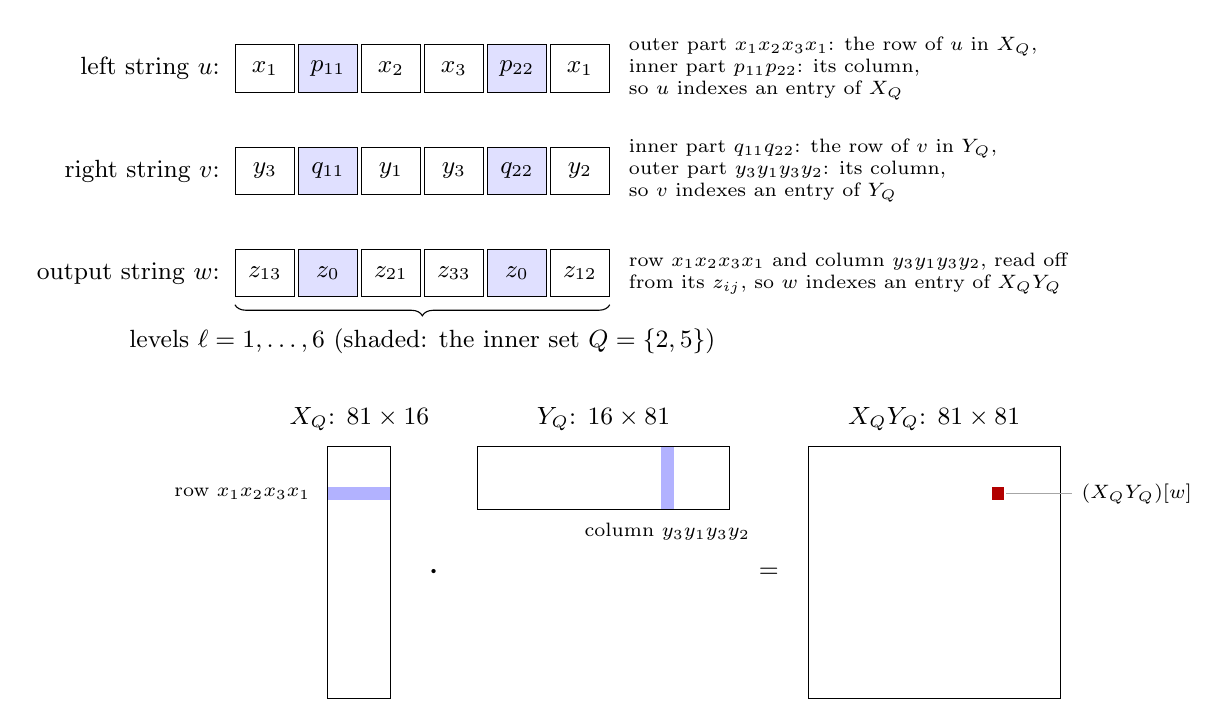
\begin{tikzpicture}[x=1cm,y=1cm,
  cell/.style={draw,minimum width=7.5mm,minimum height=6mm,inner sep=1pt,font=\small},
  inner/.style={cell,fill=blue!12},
  lab/.style={font=\scriptsize,anchor=west,align=left}]
\newcommand{\strrow}[3]{
  \foreach \txt/\sty [count=\k] in {#2} { \node[\sty] at (\k*0.8,#1) {$\txt$}; }
  \node[lab] at (6*0.8+0.5,#1) {#3};
}
\node[anchor=east,font=\small] at (0.35,0) {left string $u$:};
\strrow{0}{x_1/cell,p_{11}/inner,x_2/cell,x_3/cell,p_{22}/inner,x_1/cell}{outer part $x_1x_2x_3x_1$: the row of $u$ in $X_Q$,\\ inner part $p_{11}p_{22}$: its column,\\ so $u$ indexes an entry of $X_Q$}
\node[anchor=east,font=\small] at (0.35,-1.3) {right string $v$:};
\strrow{-1.3}{y_3/cell,q_{11}/inner,y_1/cell,y_3/cell,q_{22}/inner,y_2/cell}{inner part $q_{11}q_{22}$: the row of $v$ in $Y_Q$,\\ outer part $y_3y_1y_3y_2$: its column,\\ so $v$ indexes an entry of $Y_Q$}
\node[anchor=east,font=\small] at (0.35,-2.6) {output string $w$:};
\strrow{-2.6}{z_{13}/cell,z_0/inner,z_{21}/cell,z_{33}/cell,z_0/inner,z_{12}/cell}{row $x_1x_2x_3x_1$ and column $y_3y_1y_3y_2$, read off\\ from its $z_{ij}$, so $w$ indexes an entry of $X_QY_Q$}
\draw[decorate,decoration={brace,mirror,amplitude=4pt}] (0.8-0.38,-3.0) -- (0.8*6+0.38,-3.0) node[midway,below=5pt,font=\small] {levels $\ell=1,\dots,6$ (shaded: the inner set $Q=\{2,5\}$)};
\begin{scope}[shift={(1.6,-8.0)}]
\fill[blue!30] (0,3.2-0.6-0.08) rectangle (0.8,3.2-0.6+0.08);
\draw (0,0) rectangle (0.8,3.2); \node[font=\small] at (0.4,3.55) {$X_Q$: $81\times16$};
\node[font=\scriptsize,anchor=east] at (-0.1,3.2-0.6) {row $x_1x_2x_3x_1$};
\node[font=\Large] at (1.35,1.6) {$\cdot$};
\fill[blue!30] (1.9+2.41-0.08,2.4) rectangle (1.9+2.41+0.08,3.2);
\draw (1.9,2.4) rectangle (5.1,3.2); \node[font=\small] at (3.5,3.55) {$Y_Q$: $16\times81$};
\node[font=\scriptsize,anchor=north] at (1.9+2.41,2.35) {column $y_3y_1y_3y_2$};
\node[font=\small] at (5.6,1.6) {$=$};
\draw (6.1,0) rectangle (9.3,3.2); \node[font=\small] at (7.7,3.55) {$X_QY_Q$: $81\times81$};
\fill[red!70!black] (6.1+2.41-0.08,3.2-0.6-0.08) rectangle (6.1+2.41+0.08,3.2-0.6+0.08);
\draw[gray!70] (6.1+2.41+0.1,3.2-0.6) -- (9.45,3.2-0.6);
\node[font=\scriptsize,anchor=west] at (9.45,3.2-0.6) {$(X_QY_Q)[w]$};
\end{scope}
\end{tikzpicture}
\caption{From strings to matrix entries, for $L=6$ and $m=2$. A string whose inner set is $Q=\{2,5\}$ has an inner variable ($p$, $q$, or $z_0$) at the two levels of $Q$ and an outer one at the other four. One run of $\Full$ computes all $\binom62=15$ products $X_QY_Q$, one for each subset $Q$ of size $2$.}
\label{fig:strings}
\end{figure}

\begin{lemma}\label{lem:correct}
For the input arrays $a,b$ above and every output string $w$ whose inner set $Q$ has exactly $m$ elements,
\begin{equation}\label{eq:sum}
\Mult(a,b)[w]\;=\;(X_QY_Q)[w] .
\end{equation}
\end{lemma}

\begin{proof}
By Lemma~\ref{lem:mult}, $\Mult(a,b)[w]$ is the sum, over all left strings $u$ and right strings $v$, of $\gamma(u_1,v_1,w_1)\cdots\gamma(u_L,v_L,w_L)\,a[u]b[v]$, where $\gamma(s,t,z)$ is the coefficient of $stz$ in $G+E$. We determine which summands can be nonzero. First, $a[u]b[v]\ne0$ requires the inner sets of $u$ and $v$ to have exactly $m$ elements. Next, at a level $\ell\in Q$ we have $w_\ell=z_0$, and the only monomials of $G+E$ that contain $z_0$ are the $p_{ij}q_{ij}z_0$, with coefficient $1$. So $(u_\ell,v_\ell)=(p_{ij},q_{ij})$ for some $i,j$. Thus $u$ and $v$ have an inner variable at every level of $Q$, and their inner sets are therefore exactly $Q$. Finally, at a level $\ell\notin Q$ we have $w_\ell=z_{ij}$ for some $i,j$, and $u_\ell$ and $v_\ell$ are outer. The only monomial of $G+E$ that contains $z_{ij}$ and no inner variable is $x_iy_jz_{ij}$, with coefficient $1$, so $(u_\ell,v_\ell)=(x_i,y_j)$.

Hence, the summands that remain are those where $u$ has inner set $Q$, the row $r$ of $w$ as its outer part, and some inner part $\pi$, and where $v$ has inner set $Q$, the column $c$ of $w$ as its outer part, and the inner part $\pi'$ with the same indices as $\pi$. There is one such summand for each of the $D$ strings $\pi$, and its coefficient is $1$. Their sum is $\sum_\pi X_Q[r,\pi]\,Y_Q[\pi',c]=(X_QY_Q)[w]$.
\end{proof}

To summarize: one run of $\Full$, which uses $10^L$ multiplications, computes all $K$ of the products $X_QY_Q$. The $K$ products can be completely independent: we are free to plug in any choices for $X_Q$ and $Y_Q$ and the algorithm will give us all $K$ products. In the next subsection we will end up plugging in the same matrix for different copies $X_Q$ (and $Y_Q$). 



\subsubsection{\texorpdfstring{Tiling the $N\times D\times N$ product by products of shape $N_0\times D\times N_0$}{Tiling the N x D x N product by products of shape N0 x D x N0}}\label{sec:tiling}

We now use our algorithm, which performs $K$ simultaneous multiplications of an $\Nz \times D$ matrix with a $D \times \Nz$ matrix, in order to do a single multiplication of an $N \times D$ matrix $X$ with a $D \times N$ matrix $Y$. For our parameter setting, $N \gg \Nz$, so we can do this with a simple tiling approach. Tiling enlarges only the outer dimensions, so it handles a smaller inner dimension than Coppersmith's algorithm from the same identity (at best $D\approx N^{0.1204}$ rather than $N^{0.1402}$~\cite{Cop82}). We use it because each entry of $XY$ is then a single output of a single run of $\Full$, rather than a linear combination of many outputs as in Coppersmith's algorithm. We will take advantage of this in our algorithm below (Section~\ref{sec:sparse}).

We cut $X$ into \defn{row blocks} of $\Nz$ consecutive rows and $Y$ into \defn{column blocks} of $\Nz$ consecutive columns. Thus, $XY$ consists of all the products of a row block by a column block, each an $\Nz\times D$ by $D\times\Nz$ product, and one run of $\Full$ computes $K$ such products at once. We use each run on a $K_0\times K_0$ grid of block products, where $K_0:=\lfloor\sqrt K\rfloor$: we group the row blocks into \defn{bands} of $K_0$ consecutive blocks, and similarly the column blocks, and we call a row band together with a column band a \defn{tile} (Figure~\ref{fig:tiling}). Each tile is one run of $\Full$. We fix $K_0^2\le K$ distinct subsets of $\{1,\dots,L\}$ of size $m$, one for each block product of the grid, the same in every tile. In a tile, let $X_Q$ and $Y_Q$ be the row block and the column block of the block product with subset $Q$, and let $X_Q=Y_Q=0$ for the other subsets $Q$. Then one run of $\Full$ computes all $K_0^2$ block products of the tile (Lemma~\ref{lem:correct}), and running it on every tile computes all of $XY$.

We pair the blocks in a grid like this, rather than arbitrarily, so that the left input array of a tile depends only on its row band and the right one only on its column band. This will let us share their encodings among tiles in Section~\ref{sec:encoders} below. (To make the bands fit, we first pad $N$ to a multiple of $K_0\Nz$ with zero rows of $X$ and zero columns of $Y$, which at most doubles $N$ since $N\ge K_0\Nz$, as we will see in Section~\ref{sec:proof}.)

Before moving on, let us compute the number of operations performed by this algorithm. Let $\Cm:=K\Nz^2$ denote the number of output entries among all $K$ products of a tile. 
Since $K_0\ge\sqrt K/2$, there are $(N/K_0\Nz)^2\le4N^2/\Cm$ tiles. Thus, recalling the operation count of a single tile from Section~\ref{sec:recursion}, the whole product takes $O\big(\tfrac{N^2}{\Cm}\,L\cdot10^L\big)$ operations, that is, $O(L\cdot10^L/\Cm)$ per entry of $XY$. One can calculate that this is $N^2\,\mathrm{poly}(L)$ in total when $L=10m$, but about $N^2D^{0.2}$ for our choice $L=19m$. We nonetheless choose $L=19m$, and in Section~\ref{sec:counts} below we explain why this is needed for our sparsity arguments.

\begin{figure}[tb]
\centering
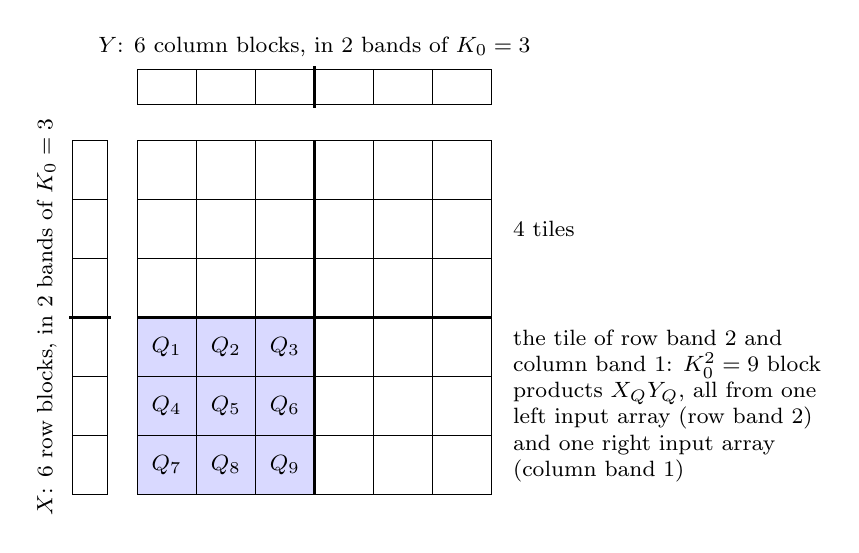
\begin{tikzpicture}[x=0.75cm,y=0.75cm,font=\footnotesize]
\draw (1.5,4.3) rectangle (7.5,4.9);
\foreach \i in {1,...,5} \draw (1.5+\i,4.3) -- (1.5+\i,4.9);
\draw[very thick] (4.5,4.25) -- (4.5,4.95);
\node[anchor=south] at (4.5,4.95) {$Y$: $6$ column blocks, in $2$ bands of $K_0=3$};
\draw (0.4,-2.3) rectangle (1.0,3.7);
\foreach \i in {1,...,5} \draw (0.4,3.7-\i) -- (1.0,3.7-\i);
\draw[very thick] (0.35,0.7) -- (1.05,0.7);
\node[rotate=90,anchor=south] at (0.3,0.7) {$X$: $6$ row blocks, in $2$ bands of $K_0=3$};
\fill[blue!15] (1.5,-2.3) rectangle (4.5,0.7);
\draw (1.5,-2.3) rectangle (7.5,3.7);
\foreach \i in {1,...,5} { \draw (1.5+\i,-2.3) -- (1.5+\i,3.7); \draw (1.5,3.7-\i) -- (7.5,3.7-\i); }
\draw[very thick] (1.5,0.7) -- (7.5,0.7);
\draw[very thick] (4.5,-2.3) -- (4.5,3.7);
\foreach \i/\j/\t in {0/0/1,1/0/2,2/0/3,0/1/4,1/1/5,2/1/6,0/2/7,1/2/8,2/2/9}
  \node at (2+\i,0.2-\j) {$Q_{\t}$};
\node[anchor=west,align=left] at (7.7,-0.8) {the tile of row band $2$ and\\ column band $1$: $K_0^2=9$ block\\ products $X_QY_Q$, all from one\\ left input array (row band $2$)\\ and one right input array\\ (column band $1$)};
\node[anchor=west,align=left] at (7.7,2.2) {$4$ tiles};
\end{tikzpicture}
\caption{The tiling, drawn for $N=6\Nz$ and $K_0=3$. A block product, a row block of $X$ times a column block of $Y$, holds $\Nz^2$ entries of $XY$. A tile, a band of $K_0$ row blocks together with a band of $K_0$ column blocks, is one run of $\Full$, which computes its $K_0^2\le K$ block products, each with its own subset $Q$ ($Q_1,\dots,Q_9$ shown in the highlighted tile).}\label{fig:tiling}
\end{figure}

\subsection{Extracting only the desired entries}\label{sec:sparse}

In this subsection, we present the main new idea of this paper. Our goal is now to compute only the wanted entries of $XY$, i.e., those at the positions in $W$, which is a set of size $|W| \leq N^2/\sqrt D$. We will modify the algorithm of Section~\ref{sec:full} in two ways. First, we will observe that the encoding (step~(2)) of each input array depends only on that array and not the other, and that each input array is shared by many tiles (defined in Section~\ref{sec:tiling}), so we can compute each encoding only once and share it among those tiles (Section~\ref{sec:encoders}). Second, we will prune the recursion tree for the multiplication and decoding steps (steps~(3)~and~(4)), by skipping a recursive call whenever none of its outputs leads to an output entry from $W$ (Section~\ref{sec:prune}). Finally we will analyze the algorithm by counting the leaves that are reached (Section~\ref{sec:counts}), and adding up the costs (Section~\ref{sec:proof}).

\subsubsection{Sharing the encoding}\label{sec:encoders}

The two numbers $\Phi_\tau(a)$ and $\Psi_\tau(b)$ multiplied at a leaf $\tau$ depend on $a$ alone and on $b$ alone, respectively, so we will compute them once per input array rather than once per tile. The \defn{encoding} of $a$ is the array of the $10^L$ numbers $\Phi_\tau(a)$, indexed by the leaves $\tau$. This is the array that the encoding steps of $\Full$ compute from $a$. To compute it, we run $\Full$ with $b$ left out and without step~(4): by Lemma~\ref{lem:recursion}, the left number at the leaf $\tau$ is $\Phi_\tau(a)$, and the leaf stores it. This takes $O(10^L)$ operations, the cost of the encoding in Section~\ref{sec:recursion}. The encoding of $b$, the array of the numbers $\Psi_\tau(b)$, is computed in the same way.

We compute the encodings of the input arrays of all row bands and all column bands (defined in Section~\ref{sec:tiling}), $2N/K_0\Nz$ arrays of $10^L$ numbers in all, and every tile reads its two encodings from these. It is important that these encodings are shared, since an encoding has $10^L=(9+1)^L$ numbers, more than the $\Cm=\binom Lm9^{L-m}$ entries of the $K$ products of a tile, so encoding every tile separately would cost more than one operation per entry of the entire matrix product (even before focusing on $W$). Since each encoding is computed only once per band, the $2N/K_0\Nz$ encodings are used by all $(N/K_0\Nz)^2$ tiles. Each one costs $O(10^L)$, independently of $W$. The assumption $N\ge D^{18}$ makes this cost negligible (as we will compute in Section~\ref{sec:proof}). 

\subsubsection{Skipping the calls that are not needed}\label{sec:prune}

Once the encodings are computed as above, we can skip that phase of $\Full$. Instead, each leaf reads its two numbers from the encodings, and each call only performs the decoding of step~(4). We now modify $\Full$ so that each call computes only the outputs that are wanted from it, i.e., the outputs that lead to entries in $W$. We will implement this by passing to each call the set $S$ of the outputs that are wanted from it.

More precisely, the outputs of the vertex $\tau_1\cdots\tau_k$ (defined in Section~\ref{sec:recursion}) are indexed by output strings of length $L-k$, and $S$ is a set of such strings. If $U$ is the set passed to the root (in the final algorithm, this will be the set of output strings of the wanted entries of the tile), we will see in Lemma~\ref{lem:prune} that $S$ will consist of the suffixes $w_{k+1}\cdots w_L$ of the strings $w\in U$ to which the vertex contributes (as defined in Section~\ref{sec:whatit}). 
Sets of output strings have slices like arrays (see Section~\ref{sec:recursion}): for a set $S$ of output strings and an output variable $z$, the slice $S_z$ is the set of output strings $w'$ with $zw'\in S$, and an array on $S$ assigns an integer to each string of $S$.

Our modified version of the recursive algorithm $\Full$, which we call $\Pruned$, is as follows.

\medskip
\noindent\begin{minipage}[t]{\linewidth}
$\Pruned_{\tau_1\cdots\tau_k}(S)$, for a set $S$ of output strings of length $L-k$, returns the array returned by the vertex $\tau_1\cdots\tau_k$ of $\Full$, restricted to the strings in $S$:
\begin{enumerate}[label=(\arabic*),nosep]
\item If $k=L$, then look up $\Phi_\tau(a)$ and $\Psi_\tau(b)$ from the precomputed encodings (Section~\ref{sec:encoders}) and return $\Phi_\tau(a)\,\Psi_\tau(b)$ for the leaf $\tau=\tau_1\cdots\tau_L$.
\item For each term $\lambda$ of Sch\"onhage's identity, let $S_\lambda$ be the union of the slices $S_z$ over the $z$ to which $\lambda$ contributes, i.e., $S_{P_{ij}}:=S_{z_{ij}}\cup S_{z_0}$ and $S_{P_0}:=S_{z_0}$.
\item For each term $\lambda$ of Sch\"onhage's identity with $S_\lambda\ne\emptyset$, compute $C_\lambda:=\Pruned_{\tau_1\cdots\tau_k\lambda}(S_\lambda)$, an array on $S_\lambda$.
\item Return the array $c$ on $S$ whose slices are $c_{z_{ij}}:=C_{P_{ij}}$ and $c_{z_0}:=\sum_\lambda C_\lambda$, restricted to $S_{z_{ij}}$ and to $S_{z_0}$. (These restrictions make sense, since $S_{z_{ij}}\subseteq S_{P_{ij}}$ and $S_{z_0}\subseteq S_\lambda$ for every $\lambda$, by step~(2).)
\end{enumerate}
\end{minipage}
\medskip

Let us confirm which leaves $\Pruned$ visits. Recall from~\eqref{eq:multdef} that $\Mult(a,b)[w]$ is the sum of $\Phi_\tau(a)\Psi_\tau(b)$ over the leaves contributing to $w$ (as defined in Section~\ref{sec:whatit}), i.e., those that choose $P_{ij}$ at every level where $w$ has $z_{ij}$, and may choose any term at levels where $w$ has $z_0$. For a set $U$ of output strings of length $L$, we write $\Leaves(U)$ for the set of leaves that contribute to some output string of $U$.

\begin{lemma}\label{lem:prune}
Let $a$ and $b$ be input arrays, and let $U$ be a set of output strings of length $L$. Called at the root, $\Pruned(U)$ returns $\Mult(a,b)$ restricted to $U$. The leaves it visits are exactly those of $\Leaves(U)$, and the sets passed to the calls it makes have total size at most $(L+1)\,|\Leaves(U)|$.
\end{lemma}

\begin{proof}
The values are correct by induction on $L-k$: each $C_\lambda$ is the array of the corresponding child of $\Full$ restricted to $S_\lambda$, so step~(4) is step~(4) of $\Full$ restricted to $S$.

Recall that $S_\lambda$ consists of the last $L-k-1$ variables of each string in $S$ such that $\lambda$ contributes to the first variable of that string. Thus, an induction on $k$ shows that the set passed to the vertex $\tau_1\cdots\tau_k$ consists of the suffixes $w_{k+1}\cdots w_L$ of the strings $w$ of $U$ to which the vertex contributes, and furthermore that the vertex is called if and only if this set is nonempty. This means a leaf is visited if and only if it contributes to some string of $U$.

For the total size, map each suffix in the set passed to a vertex $\tau_1\cdots\tau_k$ to the leaf that extends $\tau_1\cdots\tau_k$ by picking $P_{ij}$ at the levels where the suffix has $z_{ij}$ and by picking $P_0$ where it has $z_0$. By the previous paragraph, the vertex contributes to some string $w$ of $U$ with this suffix, and then so does this leaf, so the leaf is in $\Leaves(U)$. The leaf determines the vertex and the suffix. This means the sets passed to the vertices at each of the $L+1$ depths have total size at most $|\Leaves(U)|$.
\end{proof}

In other words, each call is made at most once, no matter how many strings of $U$ depend on it, and the running time depends on the size of the union of the sets of leaves contributing to the strings of $U$, rather than the sum of their sizes. It remains to bound this union.

\subsubsection{Few leaves contribute to a sparse set of entries}\label{sec:counts}

In our final algorithm, which we present below in Section~\ref{sec:proof}, the set $U$ passed to $\Pruned$ will consist only of the output strings we have been focusing on, i.e., output strings of length $L$ whose inner sets (defined in Section~\ref{sec:defs}) have exactly $m$ elements, so that they index the entries of the products $X_QY_Q$ (Lemma~\ref{lem:correct}). There are $\Cm=\binom Lm9^{L-m}=K\Nz^2$ such output strings (with $\Cm$ as defined in Section~\ref{sec:tiling}), and in this subsection all output strings are of this kind.

Our focus in this subsection is on counting how many leaves the $\Pruned$ algorithm visits. A single output string has $10^m=D^{\log_410}\approx D^{1.66}$ leaves contributing to it. This may appear problematic, since it is more than the $D$ multiplications that computing that output entry directly, as an inner product, would take. Because of this, it is important that we do not simply count the leaves of each output string of $U$ separately. Instead, we will find that most leaves contributing to an output string also contribute to many other output strings, and there are few such leaves in total.

Let us begin by classifying leaves by how many levels they choose $P_0$ at (as opposed to one of the $P_{ij}$s). As we mentioned above, the leaves contributing to an output string with inner set $Q$ are the $10^m$ leaves that choose any term at each of the $m$ levels of $Q$, but $P_{ij}$ at every level outside $Q$ where the output string has $z_{ij}$. We call the one that chooses $P_0$ at every level of $Q$ the \defn{private leaf} of the output string. The private leaf contributes to no other output string, since an output string with a different inner set requires a term other than $P_0$ at some level of $Q$, and an output string with the same inner set but a different outer part (a different $z_{ij}$ at some level outside $Q$) requires a different term there. 

To describe how close a leaf is to being a private leaf, we define the \defn{order} of a leaf as $m$ minus the number of levels at which it chooses $P_0$. A leaf contributing to an output string chooses $P_0$ only at levels of the output string's inner set, so its order is at least $0$. Since $P_0$ is the only term that serves the inner product alone, this is the classification described in the technique overview: the order of a leaf contributing to an output string is the number of levels of the string's inner set at which the leaf takes one of the terms $P_{ij}$ shared with the outer product. The only leaf of order $0$ contributing to an output string is its private leaf. Beyond this, exactly
\[
\alpha_d:=\binom md9^d
\]
leaves of order $d$ contribute to an output string, namely its private leaf with $P_0$ replaced by one of the nine other terms at $d$ of the levels of $Q$ (Figure~\ref{fig:terms}).

The total number of leaves of order $d$ in the entire recursion tree is
\[
\beta_d:=\binom{L}{m-d}9^{L-m+d}
\]
since we can choose the $m-d$ levels with $P_0$ and one of the nine other terms at every other level. In particular, $\beta_0=\binom Lm9^{L-m}=\Cm$ since the leaves of order $0$ are exactly the private leaves, and there is one per output string. A leaf of order $d$ contributes to $\binom{L-m+d}{d}$ output strings, one for each inner set of size $m$ that contains the $m-d$ levels at which it chooses $P_0$. Indeed, $\Cm\alpha_d=\beta_d\binom{L-m+d}{d}$, as both sides count the pairs of an output string and a leaf of order $d$ contributing to it. Finally, if $L=19m$, then for $1\le d\le m$ we have
\begin{equation}\label{eq:decay}
\frac{\beta_d}{\beta_{d-1}}=\frac{9(m-d+1)}{L-m+d}\le\frac{9m}{18m+1}<\frac12,\qquad\text{so}\qquad \beta_d\le2^{-d}\Cm .
\end{equation}

As in the technique overview, leaves of higher order are more numerous per output string, but each of them is shared by more output strings, and by~\eqref{eq:decay} there are fewer of them in all. Below, we count all the leaves of order $d>m/9$, whether or not they contribute to a string of $U$, and this count will be small enough since the $\beta_d$ decrease geometrically. By the ratio in~\eqref{eq:decay}, this requires $m$ to be well below $L/10$: at $m\approx L/10$, the choice that computes the whole product cheaply (Section~\ref{sec:tiling}), the ratio would be close to $1$ for small $d$, so the $\beta_d$ would stay about $\Cm$ instead of decreasing, and the count would give no saving. A small $m$ also makes $D=4^m$ small compared with $\Nz=3^{18m}$ (about $\Nz^{0.07}$), and since a tile must fit into the product, $N$ must be a large power of $D$. Together with the cost of the encodings (Section~\ref{sec:proof}), this is why Theorem~\ref{thm:main} assumes $N\ge D^{18}$.

From now on, we fix $L=19m$, so that $\Nz=3^{18m}$ and $K=\binom{19m}m$. Recall that $D=4^m$, so $2^m=\sqrt D$ and $2^{-m/9}=D^{-1/18}$.

\begin{figure}[t]
\centering
\begin{tikzpicture}[x=1cm,y=1cm,
  cell/.style={draw,minimum width=8mm,minimum height=6mm,inner sep=1pt,font=\small},
  inner/.style={cell,fill=blue!12},
  lab/.style={font=\small,anchor=west,align=left}]
\newcommand{\wordrow}[3]{
  \foreach \txt/\sty [count=\k] in {#2} { \node[\sty] at (\k*0.85,#1) {$\txt$}; }
  \node[lab] at (6*0.85+0.5,#1) {#3};
}
\node[anchor=east,font=\small] at (0.3,0) {order 0:};
\wordrow{0}{P_{13}/cell,P_0/inner,P_{21}/cell,P_{33}/cell,P_0/inner,P_{12}/cell}{the private leaf of $w$,\\ $\alpha_0=1$ leaf, contributing to $1$ output string}
\node[anchor=east,font=\small] at (0.3,-1.15) {order 1:};
\wordrow{-0.8}{P_{13}/cell,P_{ij}/inner,P_{21}/cell,P_{33}/cell,P_0/inner,P_{12}/cell}{}
\wordrow{-1.5}{P_{13}/cell,P_0/inner,P_{21}/cell,P_{33}/cell,P_{ij}/inner,P_{12}/cell}{}
\node[lab] at (6*0.85+0.5,-1.15) {$\alpha_1=\binom21\cdot9=18$ leaves,\\ each contributing to $\binom51=5$ output strings};
\node[anchor=east,font=\small] at (0.3,-2.3) {order 2:};
\wordrow{-2.3}{P_{13}/cell,P_{ij}/inner,P_{21}/cell,P_{33}/cell,P_{ij}/inner,P_{12}/cell}{$\alpha_2=\binom22\cdot81=81$ leaves,\\ each contributing to $\binom62=15$ output strings}
\draw[decorate,decoration={brace,mirror,amplitude=4pt}] (0.85*1-0.4,-2.7) -- (0.85*6+0.4,-2.7) node[midway,below=5pt,font=\small] {levels $\ell=1,\dots,6$ (shaded: the levels of $Q=\{2,5\}$)};
\end{tikzpicture}
\caption{The leaves contributing to one output string, drawn for $L=6$, $m=2$, and the output string $w=z_{13}z_0z_{21}z_{33}z_0z_{12}$ of Figure~\ref{fig:strings}. A leaf is written as the string of terms it chose, level by level. A leaf of order $d$ is the private leaf with $P_0$ replaced by one of the nine terms $P_{ij}$ (shown as a generic $P_{ij}$ in the shaded cells) at exactly $d$ levels. Leaves of higher order are more numerous per output string, but each is shared by more output strings: a leaf that chose $P_0$ at $m-d$ levels contributes to one output string for each set $Q$ of size $m$ containing those levels, $\binom{L-m+d}{d}$ of them. At $L=19m$ this makes them fewer in all, by~\eqref{eq:decay}.}
\label{fig:terms}
\end{figure}

\begin{lemma}\label{lem:count}
For every set $U$ of output strings whose inner sets have exactly $m$ elements,
\[
|\Leaves(U)|\;\le\;\sum_{d=0}^{m}\min\{|U|\alpha_d,\ \beta_d\},
\]
and if $L=19m$, then $|\Leaves(U)|\le2^{-m/9}\big(2^m|U|+2\Cm\big)$.
\end{lemma}

\begin{figure}[t]
\centering
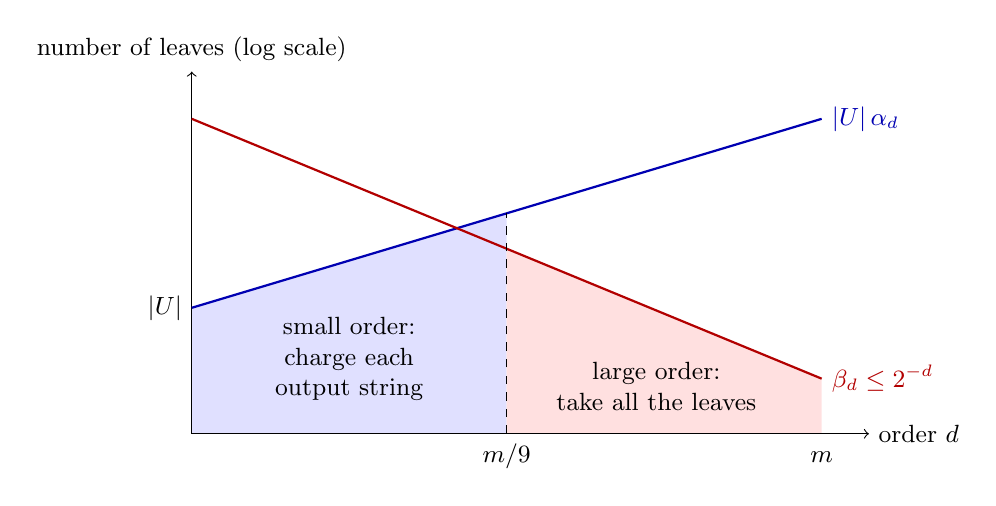
\begin{tikzpicture}[x=1cm,y=1cm]
\coordinate (A0) at (0,1.6);
\coordinate (A1) at (8,4.0);
\coordinate (B0) at (0,4.0);
\coordinate (B1) at (8,0.7);
\coordinate (XA) at (4,2.8);
\coordinate (XB) at (4,2.35);
\fill[blue!12] (A0) -- (XA) -- (4,0) -- (0,0) -- cycle;
\fill[red!12] (XB) -- (B1) -- (8,0) -- (4,0) -- cycle;
\draw[->] (0,0) -- (8.6,0) node[right,font=\small] {order $d$};
\draw[->] (0,0) -- (0,4.6) node[above,font=\small] {number of leaves (log scale)};
\draw[blue!70!black,thick] (A0) -- (A1) node[right,font=\small] {$|U|\,\alpha_d$};
\draw[red!70!black,thick] (B0) -- (B1) node[right,font=\small] {$\beta_d\le2^{-d}\Cm$};
\draw[dashed] (4,0) -- (XA);
\node[below,font=\small] at (4,0) {$m/9$};
\node[below,font=\small] at (8,0) {$m\vphantom{/9}$};
\node[left,font=\small] at (0,4.0) {$\Cm$};
\node[left,font=\small] at (0,1.6) {$|U|$};
\node[font=\small,align=center] at (2.0,0.95) {small order:\\ charge each\\ output string};
\node[font=\small,align=center] at (5.9,0.6) {large order:\\ take all the leaves};
\end{tikzpicture}
\caption{The count of Lemma~\ref{lem:count}, schematically. The leaves of order $d$ in $\Leaves(U)$ number at most $\min\{|U|\alpha_d,\,\beta_d\}$: the bound $|U|\alpha_d$ grows with $d$ up to $d\approx0.9m$ (more leaves of higher order contribute to each output string), and the bound $\beta_d$ shrinks geometrically (there are fewer leaves of higher order). The proof splits at $d=m/9$, which is not necessarily where the two bounds cross, and it bounds the total by the shaded area.}
\label{fig:count}
\end{figure}

\begin{proof}
We bound the number of leaves of order $d$ in $\Leaves(U)$ in two ways: by $|U|\alpha_d$, charging each output string of $U$ for its leaves of order $d$, and by $\beta_d$, the number of all leaves of order $d$. Since every leaf of $\Leaves(U)$ has an order $0\le d\le m$, summing the smaller of the two over $d$ gives the first inequality. (Summed on their own, $|U|\alpha_d$ gives $|U|\cdot10^m$, the cost of computing each output string of $U$ by itself, and $\beta_d$ gives less than $2\Cm$ by~\eqref{eq:decay}, the cost of computing all $\Cm$ output strings.) Neither $|U|\alpha_d$ nor $\beta_d$ depends on which output strings are in $U$.

For the second inequality, let $L=19m$. We use $|U|\alpha_d$ for the orders $d\le m/9$ and $\beta_d$ for the orders $d>m/9$ (Figure~\ref{fig:count}). The orders $d>m/9$ contribute at most $\sum_{d>m/9}\beta_d\le\Cm\sum_{d>m/9}2^{-d}<2\cdot2^{-m/9}\Cm$ by~\eqref{eq:decay}. The orders $d\le m/9$ contribute at most $|U|\sum_{d\le m/9}\binom md9^d$, and since $9^d=72^d8^{-d}\le72^{m/9}8^{-d}$ for $d\le m/9$,
\[
\sum_{d\le m/9}\binom md9^d\le72^{m/9}\sum_{d=0}^{m}\binom md8^{-d}=72^{m/9}\Big(\frac98\Big)^m=\Big(72\cdot\big(\tfrac98\big)^9\Big)^{m/9}<256^{m/9}=2^m\cdot2^{-m/9},
\]
since $72\cdot(9/8)^9<208$. Adding the two parts gives the second inequality.
\end{proof}

Since $2^m=\sqrt D$ and $2^{-m/9}=D^{-1/18}$, the second inequality of Lemma~\ref{lem:count} says that
\[
|\Leaves(U)|\;\le\;D^{-1/18}\big(\sqrt D\,|U|+2\Cm\big).
\]
Consider a tile in which $|U|=\Cm/\sqrt D$ entries are wanted. (This is the density of Theorem~\ref{thm:main}, which allows $N^2/\sqrt D$ wanted entries out of $N^2$.) Then $\sqrt D\,|U|=\Cm$, and the bound says that only $O(\Cm/D^{1/18})$ leaves contribute to the wanted entries of the tile. This is a factor $D^{1/18}$ below the number $\Cm$ of output entries of the tile, and far below the $|U|\cdot D=\Cm\sqrt D$ multiplications that computing each wanted entry directly, as an inner product, would take. Next in Section~\ref{sec:proof} we sum the number of leaves over all the tiles, and we will use the fact that the bound is linear in $|U|$, meaning the total is the same no matter how the wanted entries are spread over the tiles.

\subsubsection{Proof of Theorem~\ref{thm:main}}\label{sec:proof}

We finally put everything together to state and analyze our algorithm. As before, set $D=4^m$ and $L=19m$.

\emph{Two consequences of $N\ge D^{18}$.} We use the assumption $N\ge D^{18}$ twice, each time to check that $N$ is large enough compared with a quantity that grows exponentially in $m$. Since $D^{18}=4^{18m}$, we compare $m$-th powers by comparing their bases. 

First, the tiling of Section~\ref{sec:tiling} requires that $N\ge K_0\Nz$ so that it does not lose too much when padding, since it pads $N$ to a multiple of $K_0\Nz$. This holds: using the general bound $\binom Lm\le(eL/m)^m$, we have $K=\binom{19m}m\le(19e)^m$, so $K\Nz\le(19e\cdot3^{18})^m\le4^{18m}$, as $19e\cdot3^{18}<4^{18}$, and hence $K_0\Nz\le K\Nz\le D^{18}\le N$. This means the padding at most doubles $N$, and we continue to write $N$ for the padded size. 

Second, the encoding phase of the algorithm (Section~\ref{sec:encoders}) has a cost that does not depend on $W$ at all, and we need to ensure it is not too large. Recall that we perform $2N/K_0\Nz$ encodings, which use $O(10^L)$ operations each. To afford them within our budget of $O(2^{-m/9}N^2)$ operations, we need \begin{equation}\label{eq:enchyp}
10^L\le2^{-m/9}\,N\Nz.
\end{equation} This also holds: $10^{19}\cdot2^{1/9}/3^{18}<4^{18}$, so $10^L\cdot2^{m/9}/\Nz\le D^{18}\le N$.


\emph{The algorithm.} We compute the encodings of all row bands and column bands (Section~\ref{sec:encoders}). Each wanted position $(I,J)\in W$ lies in one tile $T$ and is indexed by one output string of $T$, the string whose inner set is the subset $Q$ of the block product containing $(I,J)$ and whose row and column are those of $(I,J)$ within that block product (Sections~\ref{sec:defs} and~\ref{sec:tiling}). For each tile $T$, let $W_T$ be the set of the output strings of the wanted positions in $T$. Then, for each tile $T$ with $W_T\ne\emptyset$, we run $\Pruned(W_T)$, and report, for each $(I,J)\in W$, the value at its output string. This is correct by Lemmas~\ref{lem:correct} and~\ref{lem:prune}.

\emph{The cost.} By~\eqref{eq:enchyp}, the encodings cost $(2N/K_0\Nz)\cdot O(10^L)=O(2^{-m/9}N^2)$ operations. Each position of $W$ lands in one set $W_T$, so $\sum_T|W_T|\le|W|\le N^2/\sqrt D=2^{-m}N^2$, and there are at most $4N^2/\Cm$ tiles, so $\sum_T\Cm\le4N^2$. A call of $\Pruned$ with a set $S$ takes $O(L|S|)$ operations, since each of its steps handles each string of $S$ a constant number of times and a string has length $L$ (we store the sets as sorted lists, so that a slice is a segment and a union of slices is a merge). By Lemma~\ref{lem:prune}, the total number of operations per leaf of $\Leaves(W_T)$ is thus $O(L^2)=O(\log^2\!D)$. Thus, by Lemma~\ref{lem:count} summed over the tiles, the pruned recursions use
\[
O\Big(L^2\sum_T|\Leaves(W_T)|\Big)\;\le\;O\Big(L^2\,2^{-m/9}\Big(2^m|W|+2\sum_T\Cm\Big)\Big)\;=\;O(L^2\,2^{-m/9}N^2)
\]
operations, no matter how $W$ is distributed among the tiles. The remaining minutiae, which list the $K_0^2$ subsets, locate the output strings, and sort the sets $W_T$, take $O(L)$ operations per subset, per tile, and per position of $W$, which is $O(L\,2^{-m/9}N^2)$ in all (as $K\le N$, there are at most $4N^2/\Nz$ tiles, $|W|\le2^{-m}N^2$, and $N,\Nz\ge2^{m/9}$). Finally, since $L=19\log_4D$ and $2^{-m/9}=D^{-1/18}$, the total operation count is $O(N^2\log^2\!D/D^{1/18})$, as desired.

\emph{Word size.} Every number the algorithm handles is an integer of magnitude $N^{O(1)}$. The input entries are of this size, by assumption. Every number in an encoding, or formed on the way to one, is a $\pm1$ combination of at most $7^L$ input entries, as step~(2) only adds and subtracts slices, and every value computed by $\Pruned$ is a sum of at most $10^L$ products of two encoded numbers (Lemma~\ref{lem:recursion}), where $7^L\le10^L\le N^2$ by~\eqref{eq:enchyp}. Indices and list positions are at most the number of words in use, also $N^{O(1)}$. Hence every integer has $O(\log N)$ bits, as desired. \qed

\begin{remark}[comparison with related techniques]
Prior work on matrix multiplication typically counts only multiplications, since they are usually a dominant cost for the algorithm, whereas in our algorithm, the additions need to be dealt with carefully. Our encodings (Section~\ref{sec:encoders}) are Yates' algorithm for Kronecker powers~\cite{Yat37,Goo58}, as is standard in recursive matrix multiplication algorithms. The pruned recursion of Section~\ref{sec:prune} is an analog of FFT pruning~\cite{Mar71,SB93}, of trimmed M\"obius inversion~\cite{BHKK10}, and, transposed, of sparse evaluation of Kronecker-power circuits~\cite{AL25}, which builds on~\cite{Wil24}. The new part along these lines in this paper is the count of Section~\ref{sec:counts}, which shows that the pruned recursion visits few leaves.
\end{remark}
